\section{Example Use Cases}
\label{sec:examples}

In this section we demonstrate how the I/O abstraction and engines described above in Section~\ref{sec:adios} can be used with different applications. These examples show how ADIOS engines can be used in different ways to accomplish the in situ processing required by a scientific campaign. The examples show how in situ can be used in both shared and separate resource configurations, and also include an example where data was streamed across the wide area network (WAN). In each example, we motivate the purpose of each scientific example and how ADIOS was used to provide the solution.

\begin{comment}
\subsection{Simple inline visualization: Owner Jong}
\todo[inline]{Majority of text from James' paper: Binning Based Data Reduction for Vector Field Data of a Particle-In-Cell Fusion Simulation.}
Visualization algorithms are particularly sensitive to I/O bandwidth, causing the community to turn to in situ techniques to alleviate this growing problem. There has been significant work and success with the in situ visualization paradigm. One of our motivating applications is XGC1, a plasma fusion simulation code that runs at scale on supercomputers. XGC1 is a gyrokinetic particle-in-cell code that is used for modeling the physics of plasmas in fusion tokamak devices. XGC1 uses a large number of particles to represent the kinetic behavior of the plasma.
Among the data sets XGC1 generating, fusion scientists are interested in looking at particle data coming from the simulation at a finer temporal fidelity than is currently possible in a post-hoc processing. In the post processing, particle data is only saved out at each of the simulation checkpoints, which only occur between every 100 and 1,000 time steps, leaving a large temporal gap. 
 
To overcome this issue of the large temporal gap, we have created a workflow for the in situ application of a data binning technique to the particle data from the simulation~\cite{kress2019binning}. The binning technique generates vectors in each of the bins that represents the speed and direction of particles within that cell’s region. Furthermore, this technique allows the scientists to tune the binning code for both specific accuracy and speed requirements by modifying the size of the binning grid, and the number of particles used to extract the vector field.

With this simple yet flexible subsampling method, we have  provided significant data reduction and in situ visualization performance so that scientists can have online particle movement information during runtime.
\end{comment}

\subsection{Strong Coupling in a Fusion Simulation}

%There are four engines in ADIOS that support strong coupling: the Sustainable Staging Transport (SST) engine, the Strong Staging Coupler (SSC) engine, the Insitu-MPI engine, and the BP4 engine. 
%The SST engine is designed to be a general-purpose staging engine that supports highly flexible configurations. Users can choose from several different underlying data transport methods, including RDMA, TCP, UDP, and shared-memory. The buffering mechanism in SST also provides several options to address different application requirements. 
%It can be configured to buffer a certain number of data steps, and when the buffer is full, it can block the writer processes, or it can delete old steps and ensure there is always space for writing newer steps. In strong coupling use cases, this buffer limit usually needs to be set to 1, thus every step is assured to be read by the readers before the application moves onto the next data step. The SST writer engine aggregates metadata for every single step, and shares it with all readers. Readers then issue remote reading operations based on the I/O pattern in metadata. Thus, it allows the I/O pattern to vary over time. SST also allows readers to disconnect and reconnect while writers keep writing. 
%While SST aims to provide the flexibility for addressing various application requirements, the fact that it does heavy metadata management work for every single step may become an overkill for use cases where metadata does not change frequently over time. For use cases where the metadata is constant across the workflow, a single aggregation operation will suffice.
%%The Insitu-MPI engine is motivated by this idea, and it is designed to only aggregate metadata once at the first data step. After that, every writer and reader knows the exact I/O pattern, and thus writers can directly send data to readers that request it using MPI send and receive through the world communicator. This requires the writer application and the reader applicaiton to be launched within a single mpiexec command in the MPMD mode. For extremely large applications that have constant I/O patterns, the Insitu-MPI engine can save a considerable amount of CPU time on metadata management, compared to the SST engine. However, the fact that it is based on the MPI MPMD mode makes it unfeasible to allow any writer or reader to join or quit dynamically at runtime. 
%
%The SSC engine is also designed for applications that have constant metadata over time. Similar to the Insitu-MPI engine, the SSC engine only aggregates metadata once at the very first step. Instead of using MPI send and receive functions in the Insitu-MPI engine, the SSC engine uses one-sided MPI communications. The one sided MPI paradigm does not require the writer and the reader to call send and receive functions in pairs, and instead, it allows a writer or reader to directly access the remote memory of another reader or writer. Thus, in very large scale coupling use cases, it saves overheads of one side waiting for the other side to complete the send and receive pair. 

%Most coupling uses cases require an N-to-M communication pattern where N and M are much smaller than the total number of staging readers and writers. Nevertheless, there is still use cases that require very large scale all-to-all communications, and for these applications, network based staging methods may not be optimal any more. Taking this into account, we developed the staging-over-file method in the BP4 engine, which allows applications to read a BP4 data set while it is being written. The advantage of the staging-over-file method over all other network based staging methods is that it needs less globally blocking function calls for sharing metadata and synchronizing step completion information. These globally blocking function calls can be very expensive in large scale all-to-all communications, and when this cost goes greater than the filesystem overhead, the staging-over-file method then outperforms the network based staging methods. 

High-Fidelity Whole Device Modeling (WDM) of Magnetically Confined Fusion Plasmas is among the most computationally demanding and scientifically challenging simulation projects.
The ten-year goal is to have a complete and comprehensive application 
that will include all the important physics components required to 
simulate a full toroidal discharge in a tokamak fusion reactor. 
The main driver is based on the strong coupling of two advanced and 
highly scalable gyrokinetic codes, XGC and GENE, where the former is a 
particle-in-cell code optimized for the treating the edge plasma while 
the other is a continuum code optimized for the core.
Applications for additional physics are intended 
to be coupled in the future, e.g. ones for material wall interactions or
for high energy particles.

In the WDM workflow, the ADIOS BPFile engine is used to save checkpoint/restart files, 
offloads variables for in situ analysis and
visualization~\cite{escience2018}. 
For in-memory data exchange, the SST and Insitu-MPI engines are used for coupling of the core and edge simulations~\cite{dominski2018}.
To date, three-dimensional field information has been
shared between XGC and GENE, but a five-dimensional distribution 
function-based coupling is now under development. Published results~\cite{escience2018, dominski2018}
have all relied on synchronous exchange, but asynchronicity will need to
be explored in order to mitigate blocking while data are not available. The ADIOS SSC engine is designed to support the asynchronous WDM coupling workflow. 
ADIOS affords both performant scalability as data sizes grow with 
increased dimensionality, as well as APIs that support asynchronous
operation.
% The synchronous exchange has been done using the Insitu-MPI and SSC ADIOS engines.
% Asyncronous coupling is being explored using the SST ADIOS engine.

\subsection{Streaming Experimental Data}

Fusion experiments provide critical information to validate and refine simulations that model complex physical processes in the fusion reactor as well as to test and validate hypotheses. 
Recent advances in sensors and imaging systems, such as sub-microsecond data acquisition capabilities and extremely fast 2D/3D imaging, allow researchers to capture very large volumes of data at high rates for monitoring and diagnostic purposes as well as post-experiment analyses. For example, JET, the world's largest magnetic confinement plasma physics experiment in the UK, is producing about 60 GB of diagnostic data per pulse~\cite{farthing2006data}. A 2-D spatial imaging system, called Electron Cyclotron Emission Imaging (ECEI), in KSTAR, Korea, alone can capture 10 GB of image data per 10 second shot~\cite{yun2010development}.

\begin{figure}[b]
\sidecaption
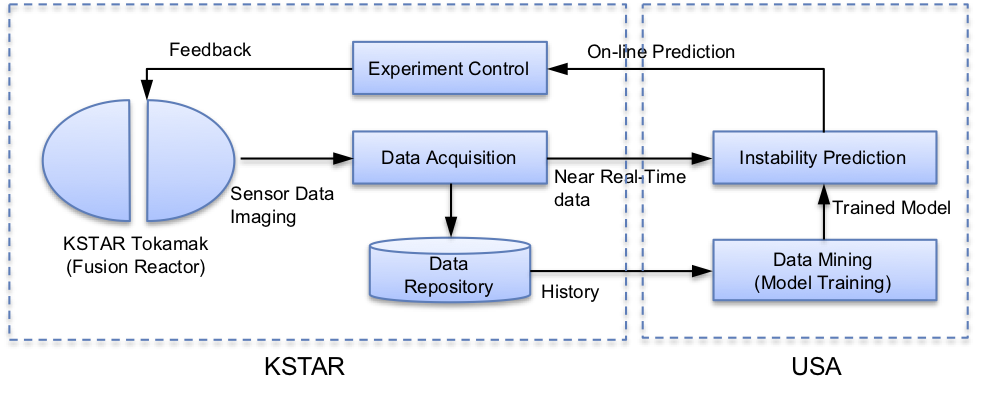
\includegraphics[width=1\linewidth]{figures/kstar-workflow.png}
\caption{Fusion instability monitoring and mitigation workflow.}
\label{fig:fusion_workflow}
\end{figure}

A system using ADIOS has been developed for KSTAR to support various data challenges by executing remote experimental data processing workflows in fusion science. It is one of the drivers for the development of the DataMan engine to support science workflows execution over the wide-area network (WAN) for near-real-time (NRT) streaming of experiment data to and from an experiment site and remote computing resource facilities. 

An example of KSTAR workflow is shown in Figure~\ref{fig:fusion_workflow}. This workflow is a multi-level workflow in that each box consists of one or more sub-workflows, each of which can be composed with ADIOS engines. One of the main goals is to stream online fusion experiment data from KSTAR in Korea to a computing facility in USA in order to perform various computational intensive analyses, such as instability prediction and disruption simulation. 
While our previous effort~\cite{choi2013icee} focused on building remote workflows with data indexing, we are currently working on composing the KSTAR workflow with DataMan. In this workflow, we use ADIOS' DataMan engine to move raw observational data as streams from Korea to the USA. Once data streams arrived in a USA computing facility, we launch a set of analysis and visualization workflows to perform denoising, segmentation, feature detection, and selection for detecting any instabilities. 
Visualization results can be delivered back to Korea for designing the next upcoming shots. 
In short, ADIOS engines enable researchers to compose and execute workflows spanning local resources and remote large-scale high performance computing facilities for NRT analysis and decision-making. 

%The volume, velocity, and variety (data elements from thousands of sensors) of KSTAR data make it extremely challenging for researchers to analyze the data only using computational resources at experiment facilities. Moreover, near-real-time (NRT) analysis and decision-making is of paramount importance in fusion experiments. 
%Researchers need ability to compose and execute workflows spanning local resources and remote large-scale high performance computing facilities.  
%Monitoring, predicting, and mitigating instabilities during an experiment need strong NRT analysis capabilities. 
%Unstable high-energy plasmas can cause serious damage to the reactor chamber, costing hundreds of millions of dollars to repair or substantial loss in productivity. 

%We have been developing an ADIOS based middleware to support various data challenges on executing experimental data processing workflows in fusion science, including development of DataMan engine in order to support science workflows execution over the wide area network (WAN) for near-real-time streaming of experiment data to and from an experiment site and remote computing resource facilities. 
%We focus on how we execute remote workflows over WAN with NRT requirement.

%An example of workflow to monitor, predict, and mitigate instabilities is shown in Figure~\ref{fig:fusion_workflow}. This workflow is a multi-level workflow in that each box consists of one or more sub-workflows. 

%To facilitate more efficient experimental work in fusion science, analysis workflows and underlying middleware infrastructure to execute them on local and remote resources should be able to handle thousands of streams of multi-dimensional sensor data within near-real time analysis constraints. 





\subsection{Interactive In Transit Visualization}
\label{sec:jaxa}
The Japan Aerospace Exploration Agency (JAXA) has implemented various ways for visualizing one of their CFD simulations, upacs-mc-LES. The visualization of CFD data consists of both batch and interactive visualization. Batch visualization is performed to create preset view images of the flowfield. Interactive visualization is conducted by interactively using Visit to understand the physics of the flowfield. While interactive visualization is not performed all the time during simulation, it is essential to have the capability to launch and attach the visualization process to the simulation when necessary, then to seamlessly detach when finished.

The agency has a heterogeneous HPC system, the Supercomputer System Generation 2 (JSS2). The main computer is a Fujitsu supercomputer with FX100 CPUs specialized for vector computations. Another cluster with x86 processors and GPUs is available for visualization and GPU-based analysis. There is a shared Lustre file system, which can be used for post-processing. An Ethernet and InfiniBand network connects the two machines, but only a portion of the nodes can communicate between the two machines. Most of the nodes can only communicate with other nodes on the internal network.

Batch visualization in post-processing is an easy way to produce movies of preset 3D visualizations on the GPU cluster, but it is stressing the file system and cannot support the largest simulations due to the I/O overhead. In situ visualization based on LibSim~\cite{libsim} is another approach, where the main computer is used to produce the images within the simulation code. In situ not only allows for producing a movie without dumping all data to disk but it also allows for interactive data exploration. ADIOS makes another approach feasible: in transit visualization where the simulation data is streamed from the main computer to another application, which in turn uses LibSim to create the visualizations. The visualization can be performed either on the main computer or on the GPU cluster (see Fig.~\ref{fig:insituJAXA_arch}). In all cases, Visit is used as the GUI for attaching to the visualization in case the user wants to interactively explore the data set.

\begin{figure}[b]
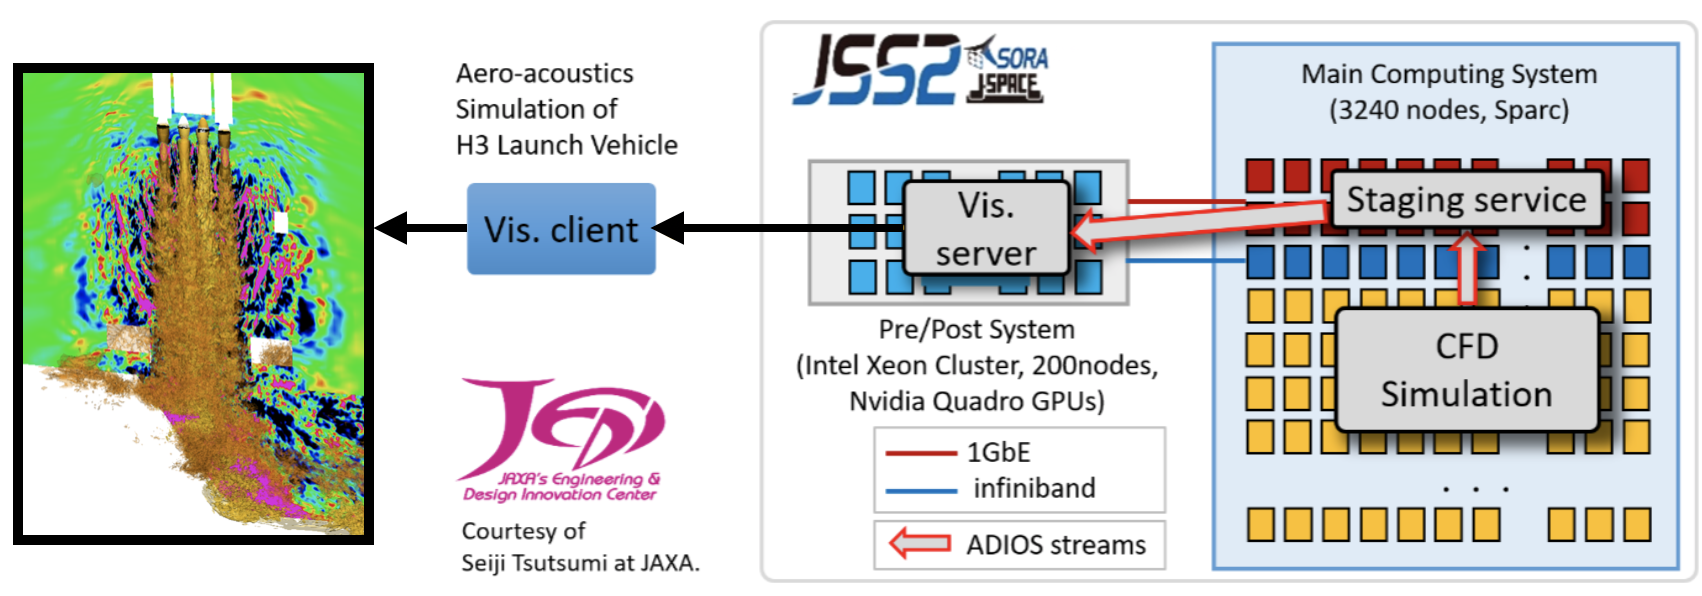
\includegraphics[width=1\linewidth]{figures/JAXA.png}
\caption{Two steps of staging of data necessary on the JAXA heterogeneous system for interactive visualization. Simulation data is staged to a concurrent staging service on nodes that have network connections to the GPU cluster. The data is further staged to the visualization server running on the GPU cluster. The visualization client then visualizes the data. The visualization on the left shows acoustic waves on the cross section and exhaust jet are visualized by normalized pressure fluctuation and iso-surface of temperature, respectively.}
\label{fig:insituJAXA_arch}
\end{figure}

The main drawback of in situ visualization with LibSim, for interactive exploration, is that the simulation process stops during interactive visualization. JAXA users want the simulation to progress with the computation while they are looking at a snapshot in time. In transit visualization using the ADIOS SST engine solves that problem and is as easy to use as in situ visualization when launching them as two separate applications together on the main computer in a single job.

Another advantage of in transit visualization (both for batch and interactive visualization) is that the simulation is not affected by the visualization process in terms of computing performance, nor by abnormal termination of the visualization process. The simulation progresses independently from the visualization and therefore the cost of visualization is amortized. On the other hand, data movement also has a cost and this offsets some of the advantages. 
As discussed in Section~\ref{sec:implications}, there are trade-offs between the in situ and in transit approaches, and it depends on the simulation size, data size and visualization cost in order to determine which approach works best. Therefore, JAXA wants to maintain and provide all approaches to visualization for its users. 

In transit visualization also provides the capability to use the GPU cluster for the visualization. The main difficulty with using a separate machine is that two jobs need to be submitted to two different machines and run at the same time.
Current job scheduling policies only support batch processing. Therefore, the only way to do interactive visualization on the GPU cluster is to submit an interactive job once the simulation is running.
This is fine for interactive visualization where the user is present. Although ADIOS makes it possible to run the visualization application immediately and let it wait for the connection to the simulation indefinitely, for a batch visualization of an overnight job, this is still a waste of resources (on the GPU cluster).

Lastly, note that using ADIOS in the simulation to output the data, the target for the data can be a concurrent application for batch visualization on the main computer, or an application on the GPU cluster for interactive/batch visualization, or it can be the Lustre file system for storing data for post-processing. The visualization application is also the same for all the three cases. It is only a matter of the runtime setup and the choice of the ADIOS Engine to run any of these cases. 
